\documentclass{beamer}

%Includes
\usepackage[utf8]{inputenc}
\usepackage[T1]{fontenc}
\usepackage{graphics}
\usepackage{graphicx}
\usepackage{subcaption}
\usepackage{eurosym}
\usepackage[francais]{babel}

%Thème
\usetheme{Warsaw}

%Template
\setbeamertemplate{footline}[page number]

%Informations de la page de garde
\title{\textbf{Projet Njord}\\ Topographie d'une zone \\ par communication avec une équipe de drones}
\author{Aigreault Clément, Henrio Jordan, Pham Chitin}
\date{16 Mars 2015}

\begin{document}
  %Page de garde
  {
    \makeatletter
    \setbeamertemplate{headline}[default]
    \def\beamer@entrycode{\vspace*{-\headheight}}
    \makeatother
    \begin{frame}
      \titlepage
    \end{frame}
  }
  
  %Introduction
  %Introduire les raisons de ce projet et qu'est-ce qu'on développe
  {
    %Permet de retirer le header ainsi que l'espace qu'il prendrait
    \makeatletter
    \setbeamertemplate{headline}[default]
    \def\beamer@entrycode{\vspace*{-\headheight}}
    \makeatother
    %Présenter les besoins
    \begin{frame}
      \frametitle{Introduction}
      \framesubtitle{Besoin}
      
      \begin{itemize}
	\item Environnements inaccessibles par l'être humain
	\item Mission d'urgence, chantier...
	\item Besoin d'un intermédiaire
      \end{itemize}
    \end{frame}

    \makeatletter
    \setbeamertemplate{headline}[default]
    \def\beamer@entrycode{\vspace*{-\headheight}}
    \makeatother
    %Expliquer que la technologie actuelle peut répondre aux besoins
    \begin{frame}
      \frametitle{Introduction}
      \framesubtitle{Ressources}
      
      \begin{itemize}
	\item Technologie à un stade intéressant
	\begin{itemize}
	  \item Robotique
	  \item Intelligence artificielle
	  \item Communication sans fil
	\end{itemize}
	\item Possibilité de "donner vie" à des machines 
	\item Une perte matérielle est moins importante qu'une perte humaine
      \end{itemize}
    \end{frame}
    
    \makeatletter
    \setbeamertemplate{headline}[default]
    \def\beamer@entrycode{\vspace*{-\headheight}}
    \makeatother
    %Présenter une solution possible
    \begin{frame}
      \frametitle{Introduction}
      \framesubtitle{Solution}
      
      \begin{itemize}
	\item Élaboration d'un réseau étoilé
	\item Le noyau : un serveur
	\item Les branches : drones volants
	\item Les drones récoltent des informations
	\item Le serveur cartographie la zone
      \end{itemize}
    \end{frame}
    
    \makeatletter
    \setbeamertemplate{headline}[default]
    \def\beamer@entrycode{\vspace*{-\headheight}}
    \makeatother
    %Schéma de la solution
    \begin{frame}
      \frametitle{Introduction}
      \framesubtitle{Solution}
      
      \begin{figure}[htbp]
	\centering
	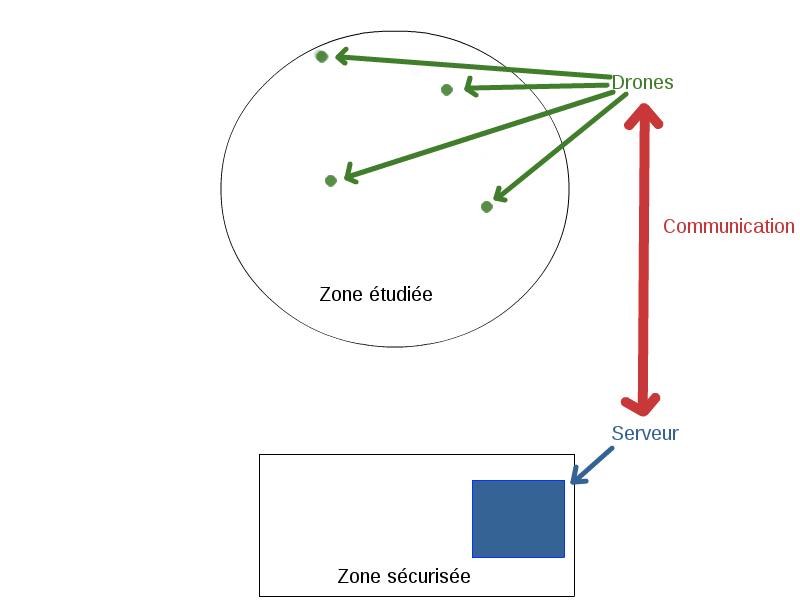
\includegraphics[scale=0.23]{img/projet_schema.png}
	\caption{Schéma du réseau}
      \end{figure}  
    \end{frame}
    
    \makeatletter
    \setbeamertemplate{headline}[default]
    \def\beamer@entrycode{\vspace*{-\headheight}}
    \makeatother
    %Présenter vulgairement notre application
    \begin{frame}
      \frametitle{Introduction}
      \framesubtitle{Application}
      
      \begin{itemize}
	\item Drones autonomes et équipés d'un capteur ultrason
	\item Communication par fréquences radio
	\item Représentation graphique de la zone en temps réel
      \end{itemize}
    \end{frame}
  }
  
  %Plan de la présentation
  %Expliquer le déroulement de la présentation
  {
    \makeatletter
    \setbeamertemplate{headline}[default]
    \def\beamer@entrycode{\vspace*{-\headheight}}
    \makeatother
    \begin{frame}
      \frametitle{Déroulement de la présentation}
      \tableofcontents[hidesubsections]
    \end{frame}
  }
  
  %Section Serveur
  %Présenter le serveur : de quoi il est constituer ? comment il fonctionne ? qu'est-ce qu'on obtient, etc...
  {
    \section{Serveur}
    
      %Re situe le cours de la présentation
      \begin{frame}
	\tableofcontents[hideothersubsections]
      \end{frame}
     
      %Sous-section Principe de fonctionnement
      %Présenter le schéma et le rôle de chaque tâche
      \subsection{Principe}
	\begin{frame}
	  \begin{itemize}
	   \item Traite les informations recoltées
	   \item Chaque drone connaît le serveur, mais pas les autres drones
	   \item Le serveur connaît tous les drones
	   \item Possibilité d'envoyer des ordres
	  \end{itemize}
	\end{frame}
      
	\begin{frame}
	  \begin{itemize}
	    \item Constitué de trois entités distinctes
	    \begin{itemize}
	      \item Communication
	      \item Sauvegarde des données
	      \item Cartographie
	    \end{itemize}
	    \item Concurrence
	    \item Limiter la perte d'informations
	  \end{itemize}
	\end{frame}
	
	\begin{frame} %Modélisation du serveur
	  \begin{figure}[htbp]
	    \centering
	    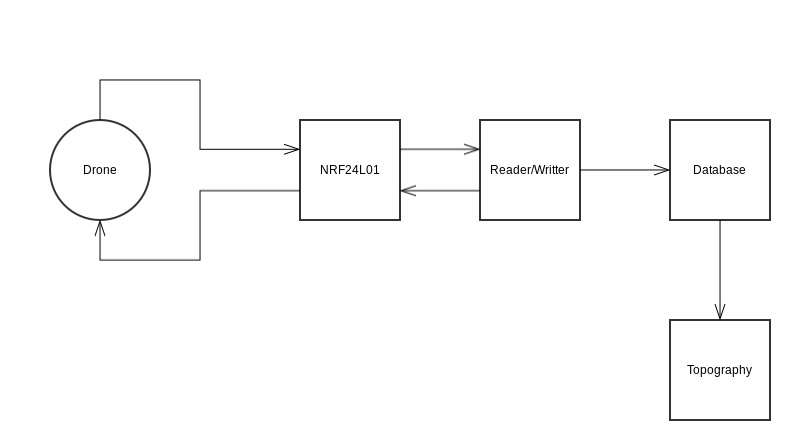
\includegraphics[scale=0.3]{img/server_model.png}
	    \caption{Modèle du serveur}
	  \end{figure}  
	\end{frame}

	\begin{frame} %Tâche 1 : Communication
	  \frametitle{Tâche 1 : Communication}
	
	  \begin{itemize}
	    \item Lit les messages des drones
	    \item Écrit sur le port série de la machine
	    \item Lit le port série
	    \item Envoie des ordres aux drones
	  \end{itemize}
	\end{frame}
	
	\begin{frame} %Tâche 2 : Sauvegarde des données
	  \frametitle{Tâche 2 : Sauvegarde des données}
	
	  \begin{itemize}
	   \item Lit le port série
	   \item Insère les messages dans la base de données (BDD)
	   \item Écrit sur le port série
	  \end{itemize}
	\end{frame}
	
	\begin{frame} %Tâche 3 : Cartographie
	  \frametitle{Tâche 3 : Cartographie}
	
	  \begin{itemize}
	    \item Lit le contenu de la BDD
	    \item Insère chaque entrée dans une matrice
	    \item Dessine le contenu de la matrice
	    \item Détermine si un ordre doit être envoyé
	  \end{itemize}
	\end{frame}

      %Sous-section Développement du serveur
      %Présenter l'implémentation de chaque tâche
      \subsection{Développement}
	\begin{frame} %Tâche 1 : Communication
	  \frametitle{Tâche 1 : Communication}
	  
	  \begin{itemize}
	    \item Utilisation d'un NRF24L01 (composant)
	    \item Implémentation en Arduino
	  \end{itemize}
	\end{frame}
	
	\begin{frame} %Tâche 2 : Sauvegarde des données
	  \frametitle{Tâche 2 : Sauvegarde des données}
	  
	  \begin{itemize}
	    \item Implémentation en Python
	    \item BDD implémentée à l'aide de Redis
	    \begin{itemize}
	      \item Utilisation simple (fonctionnement, Python)
	      \item Système robuste comme SQL inutile
	    \end{itemize}
	  \end{itemize}
	\end{frame}
	
	\begin{frame} %Tâche 3 : Cartographie
	  \frametitle{Tâche 3 : Cartographie}
	  
	  \begin{itemize}
	    \item Implémentation en Python
	    \item Utilisation de Numpy et MatPlotLib
	    \item Matrice souvent redimmensionnée
	  \end{itemize}
	\end{frame}
	
      %Sous-section Démonstration du fonctionnement
      %Montrer une impression d'écran de topographie et faire une démonstration en direct
      \subsection{Démonstration}
	\begin{frame} %Impression d'écran exemple de topographie
	  \begin{figure}[htbp]
	    \centering
	    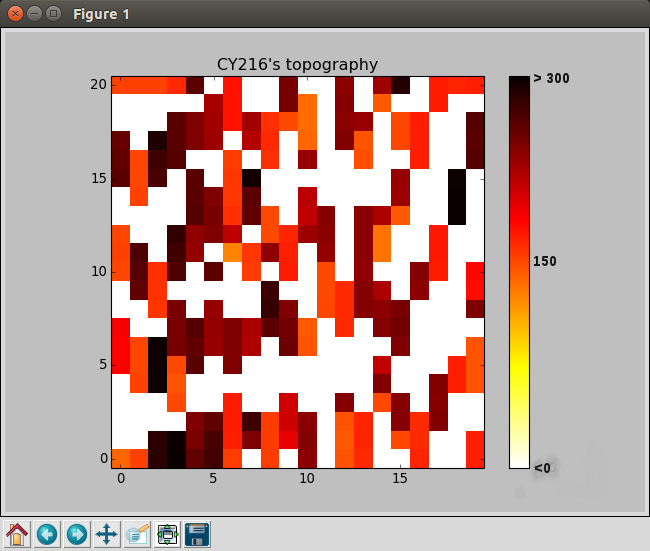
\includegraphics[scale=0.3]{img/topography_example.png}
	    \caption{Exemple de rendu de topographie}
	  \end{figure} 
	\end{frame}
	
	\begin{frame} %Démonstration en direct
	  \makebox[\linewidth]{Démonstration}\par
	\end{frame}
  }
  
  %Section Drone
  %Présenter le drone : Les composants, les librairies, le résultat final, ...
  {
    \section{Drone}
    
      %Re situe le cours de la présentation
      \begin{frame}
	\tableofcontents[hideothersubsections]
      \end{frame}
    
      %Sous-section Étude prémilinaire
      %Présenter les recherches qui ont été faites avant l'achat des composants
      \subsection{Étude préliminaire}
	\begin{frame}
	  \begin{itemize}
	    \item Réalisation du cahier des charges
	    \item État de l'art
	    \begin{itemize}
	      \item Crazyflie (BitCraze)
	      \item ARDrone (Parrot)
	      \item Phantom (DJI)
	    \end{itemize}
	    \item Plusieurs type de drones (grand/petit, rapide/lent, agile/prise de vues...)
	    \item Étape non négligeable d'un projet
	  \end{itemize}
	\end{frame}
	
	\begin{frame}
	  \begin{itemize}
	    \item Coup de coeur pour le Crazyflie de BitCraze
	    \item Pièces détachées, code source disponible, libre
	    \item Un peu cher et ne correspond pas parfaitement à notre application
	  \end{itemize}
	\end{frame}
	
	\begin{frame}
	  \begin{figure}[htbp]
	    \centering
	    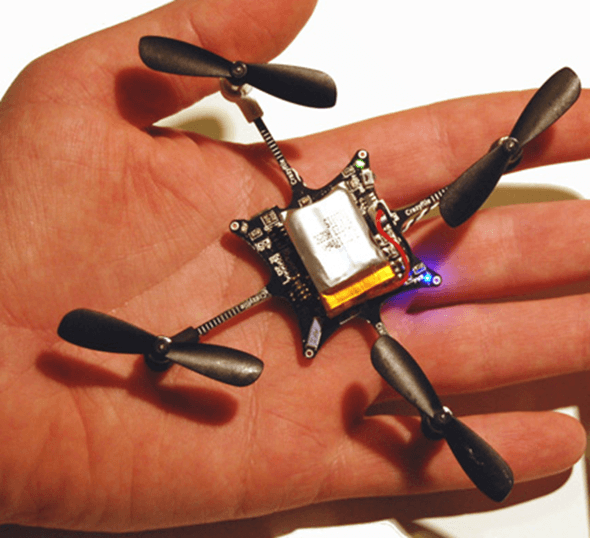
\includegraphics[scale=0.2]{img/crazyflie.png}
	    \caption{Photo du Crazyflie de BitCraze}
	  \end{figure} 
	\end{frame}

	\begin{frame}
	  \begin{itemize}
	    \item Devis
	    \item Premières estimations
	    \begin{itemize}
	      \item Poids
	      \item Puissance requise
	      \item Consommation en courant
	      \item Autonomie
	    \end{itemize}
	    \item Plus lourd que le Crazyflie mais moins cher
	  \end{itemize}
	\end{frame}
      
      %Sous-section Composants
      %Présenter les composants choisis 
      \subsection{Composants}
	\begin{frame} %Arduino
	  \frametitle{Arduino}
	
	  \begin{itemize}
	    \item Cours d'Arduino en début d'année
	    \item Micro-contrôleurs très en vogue
	    \item Similaire au C/C++
	    \item Bon marché et existe en petite taille
	  \end{itemize}
	\end{frame}
	
	\begin{frame}
	  \frametitle{Arduino}
	  
	  \begin{figure}[htbp]
	    \centering
	    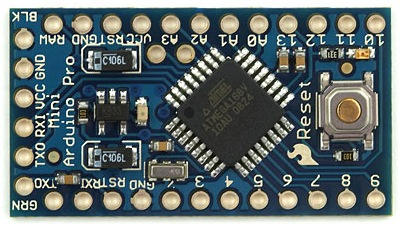
\includegraphics[scale=0.2]{img/arduinopromini.jpg}
	    \caption{Photo de l'Arduino Pro Mini}
	  \end{figure} 
	\end{frame}
	
	\begin{frame} %Gyroscope/Accéléromètre
	  \frametitle{Gyroscope/Accéléromètre}
	
	  \begin{itemize}
	    \item Besoin de stabiliser le drone
	    \item MPU-6050 très répandu, petit, bon marché et embarque un 
accéléromètre
	    \item Besoin de déterminer la position du drone dans l'espace
	    \begin{itemize}
	      \item GPS : Trop peu précis pour une salle
	      \item Triangulation : Trop coûteux, peu adapté à la problématique
	      \item Mesure de l'accélération
	    \end{itemize}
	    \item Solution non exploitable
	  \end{itemize}
	\end{frame}
	
	\begin{frame}
	  \frametitle{Gyroscope/Accéléromètre}
	
	  \begin{figure}[htbp]
	    \centering
	    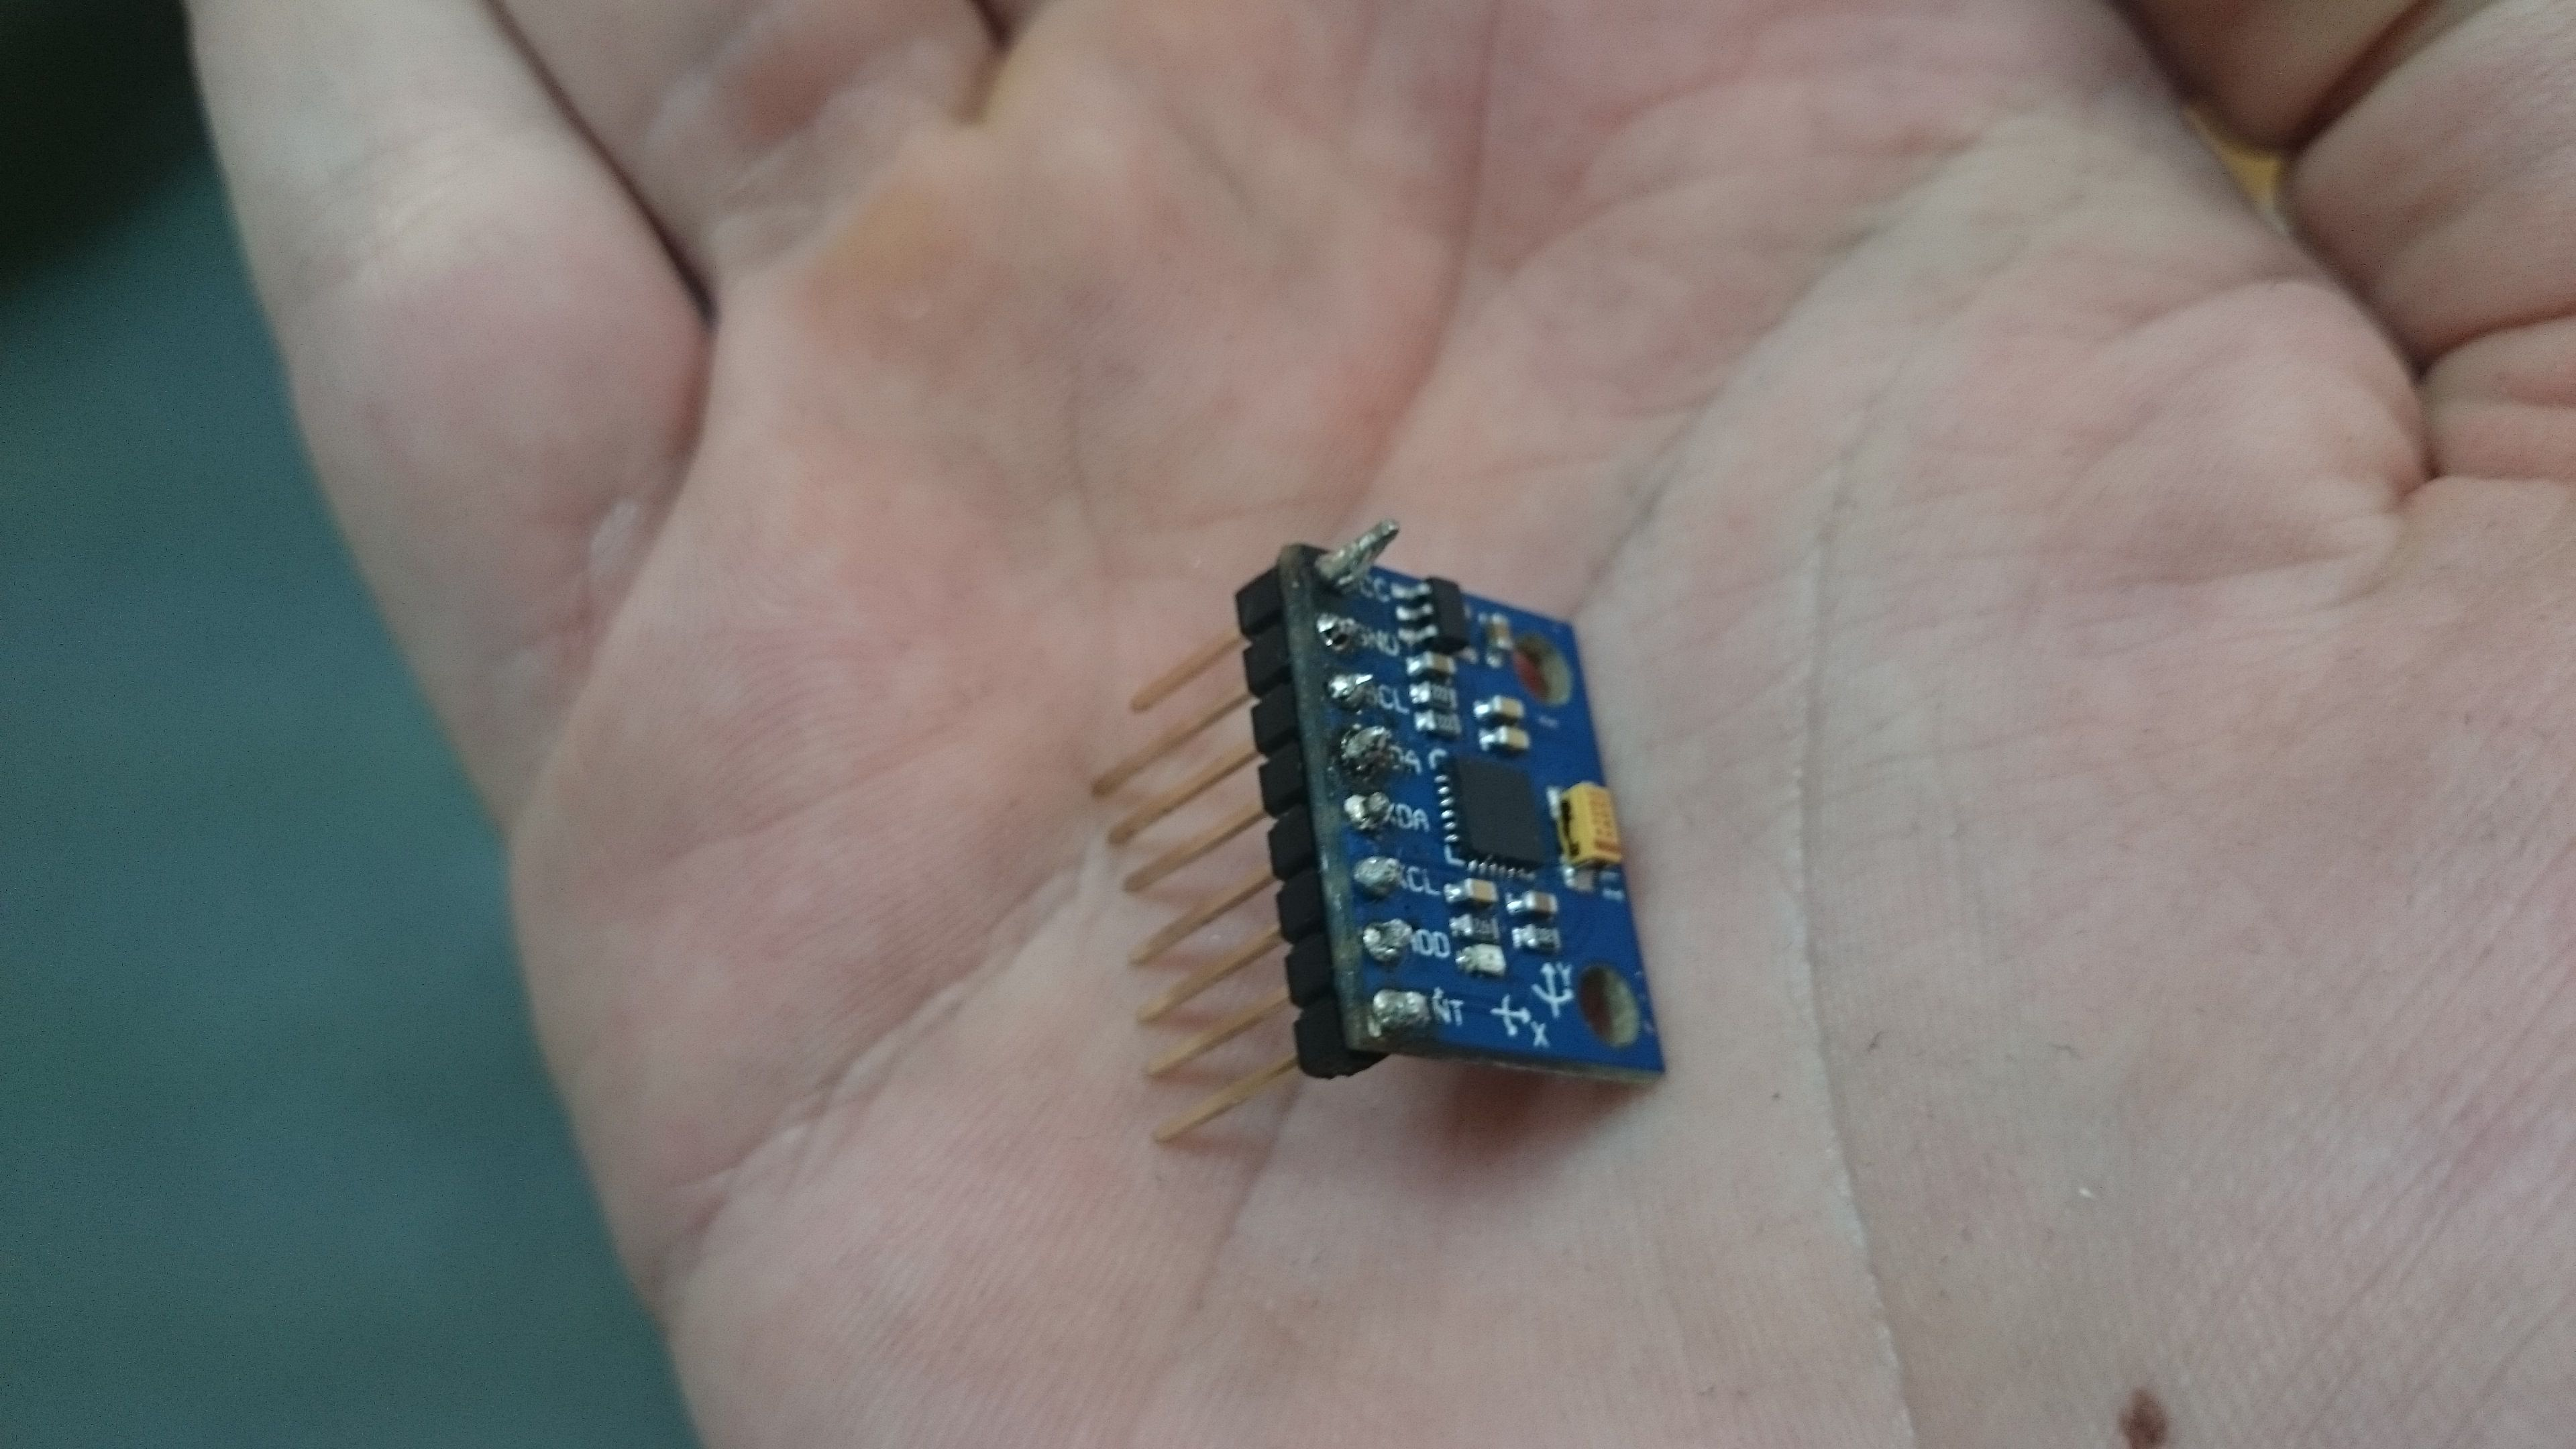
\includegraphics[scale=0.05]{img/mpu6050.jpg}
	    \caption{Photo du MPU-6050}
	  \end{figure} 
	\end{frame}
	
	\begin{frame} %Communication sans fil
	  \frametitle{Communication sans fil}
	
	  \begin{itemize}
	    \item Nombreux composants sur le marché
	    \begin{itemize}
	      \item Modules XBee : Très utilisé mais trop coûteux ($\sim$ 30 
\euro) et trop gros
	      \item Fréquence radio : Assez utilisé, bon marché ($\sim$ 0,80 
\euro) et petit
	    \end{itemize}
	    \item NRF24L01 suffisant au sein d'une même pièce
	  \end{itemize}
	\end{frame}
	
	\begin{frame}
	  \frametitle{Communication sans fil}
	
	  \begin{figure}[htbp]
	    \centering
	    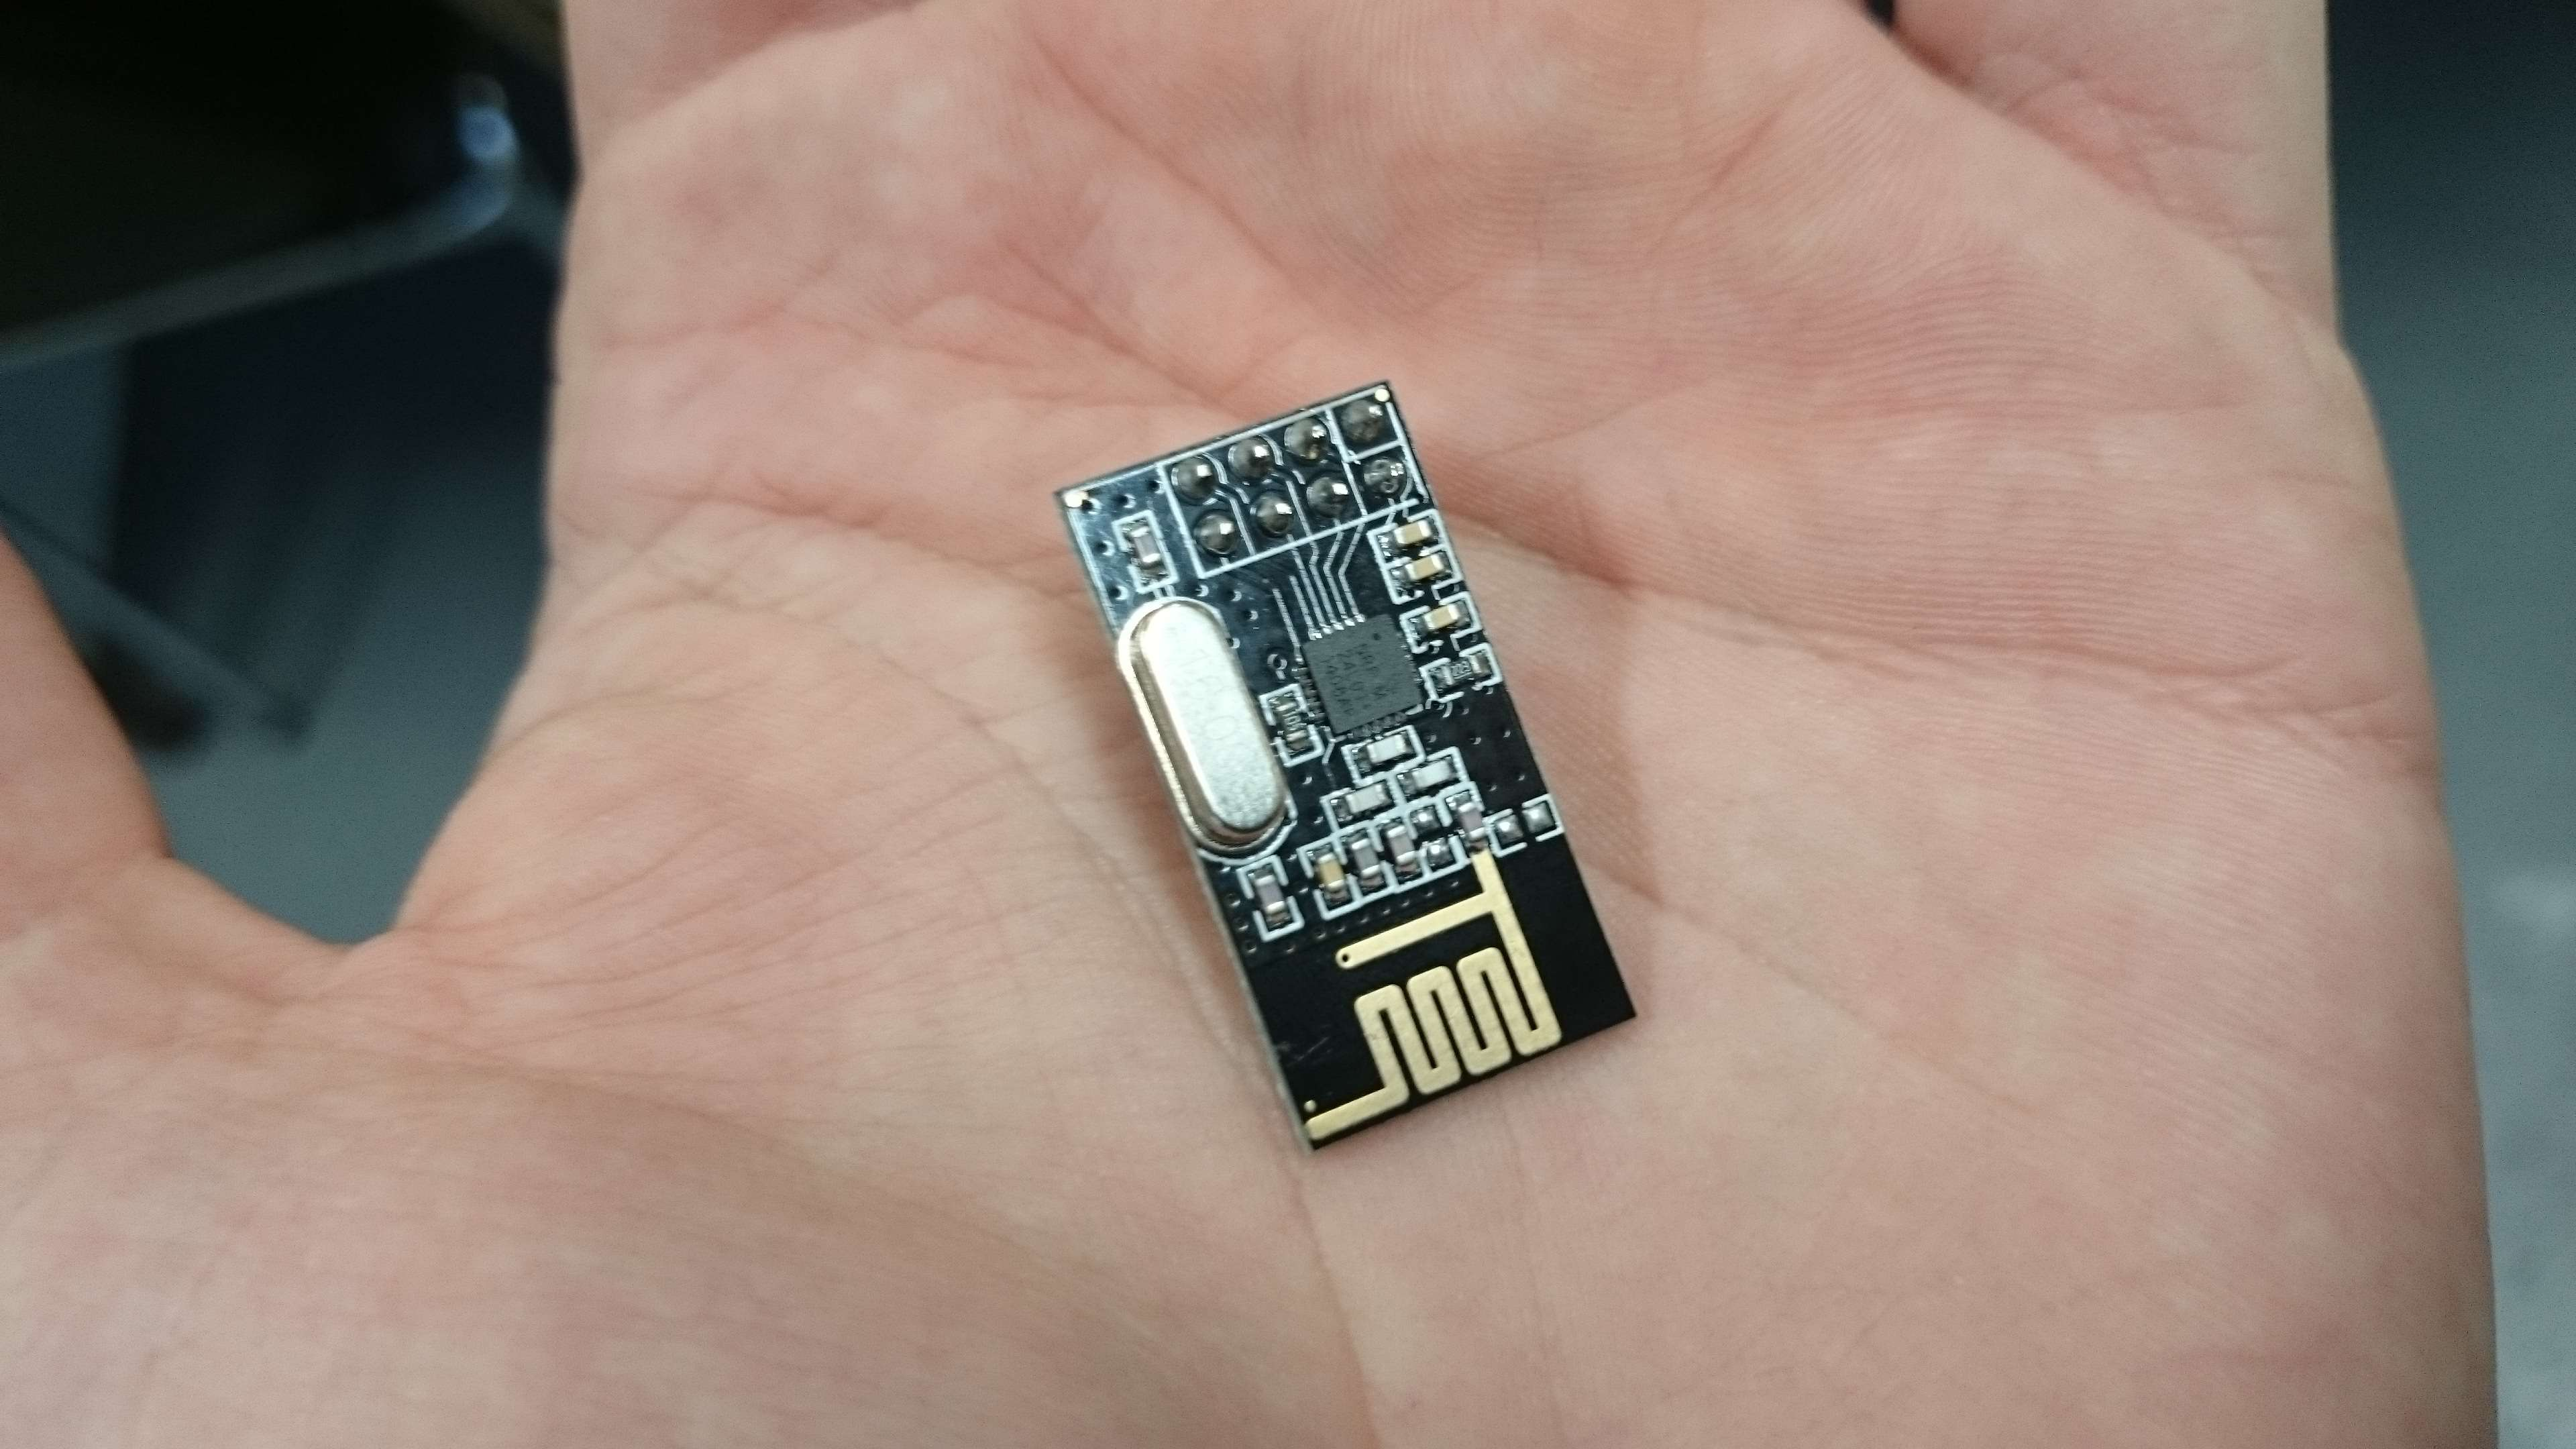
\includegraphics[scale=0.05]{img/nrf24l01.jpg}
	    \caption{Photo du NRF24L01}
	  \end{figure} 
	\end{frame}
	
	\begin{frame} %ESC
	  \frametitle{ESC}
	
	  \begin{itemize}
	    \item Electric Speed Controler(ESC)
	    \item Coûteux ($\sim$ 15 \euro / moteur)
	    \item Lourd ($\sim$ 25g / ESC)
	    \item Fabrication possible (transistor)
	  \end{itemize}
	\end{frame}
	
	\begin{frame} %Moteur, batterie, total
	  \frametitle{Moteur, batterie, total}
	
	  \begin{itemize}
	    \item Même moteurs et batterie que le Crazyflie
	    \item $\sim$ 25 \euro \space contre 120 \euro
	    \item 35g contre 19g (estimation)
	  \end{itemize}
	\end{frame}

      %Sous-section Développement et montage
      %Parler des implémentation qui on été faites
      \subsection{Développement et aquisition des pièces manquantes}
	\begin{frame} %Explication des bibliothèques
	  \begin{itemize}
	    \item Développement de bibliothèques composant avant assemblage
	    \begin{itemize}
	      \item Moteur
	      \item Communicateur radio : Surcouche de RadioHead
	      \item Gyroscope : Inspiration de Jeff Rowberg 
	    \end{itemize}
	  \end{itemize}
	\end{frame}
	
	\begin{frame} %Histoires de PCB et des fixations moteur
	  \begin{itemize}
	    \item Encore deux pièces manquantes
	    \begin{itemize}
	      \item Circuit imprimé
	      \item Fixations moteurs
	    \end{itemize}
	    \item Pas de matériel à l'EISTI, besoin d'aide extérieur
	    \item Visite au fablab de Gennevilliers
	  \end{itemize}
	\end{frame}

	\begin{frame}
	  \frametitle{Circuit imprimé}
	  
	  \begin{itemize}
	    \item Dessin du circuit à l'aide du logiciel Fritzing
	    \item Support de la part de l'ENSEA
	  \end{itemize}
	\end{frame}
	
	\begin{frame}
	  \frametitle{Circuit imprimé}
	
% 	  \begin{figure}[htbp]
% 	    \centering
% 	    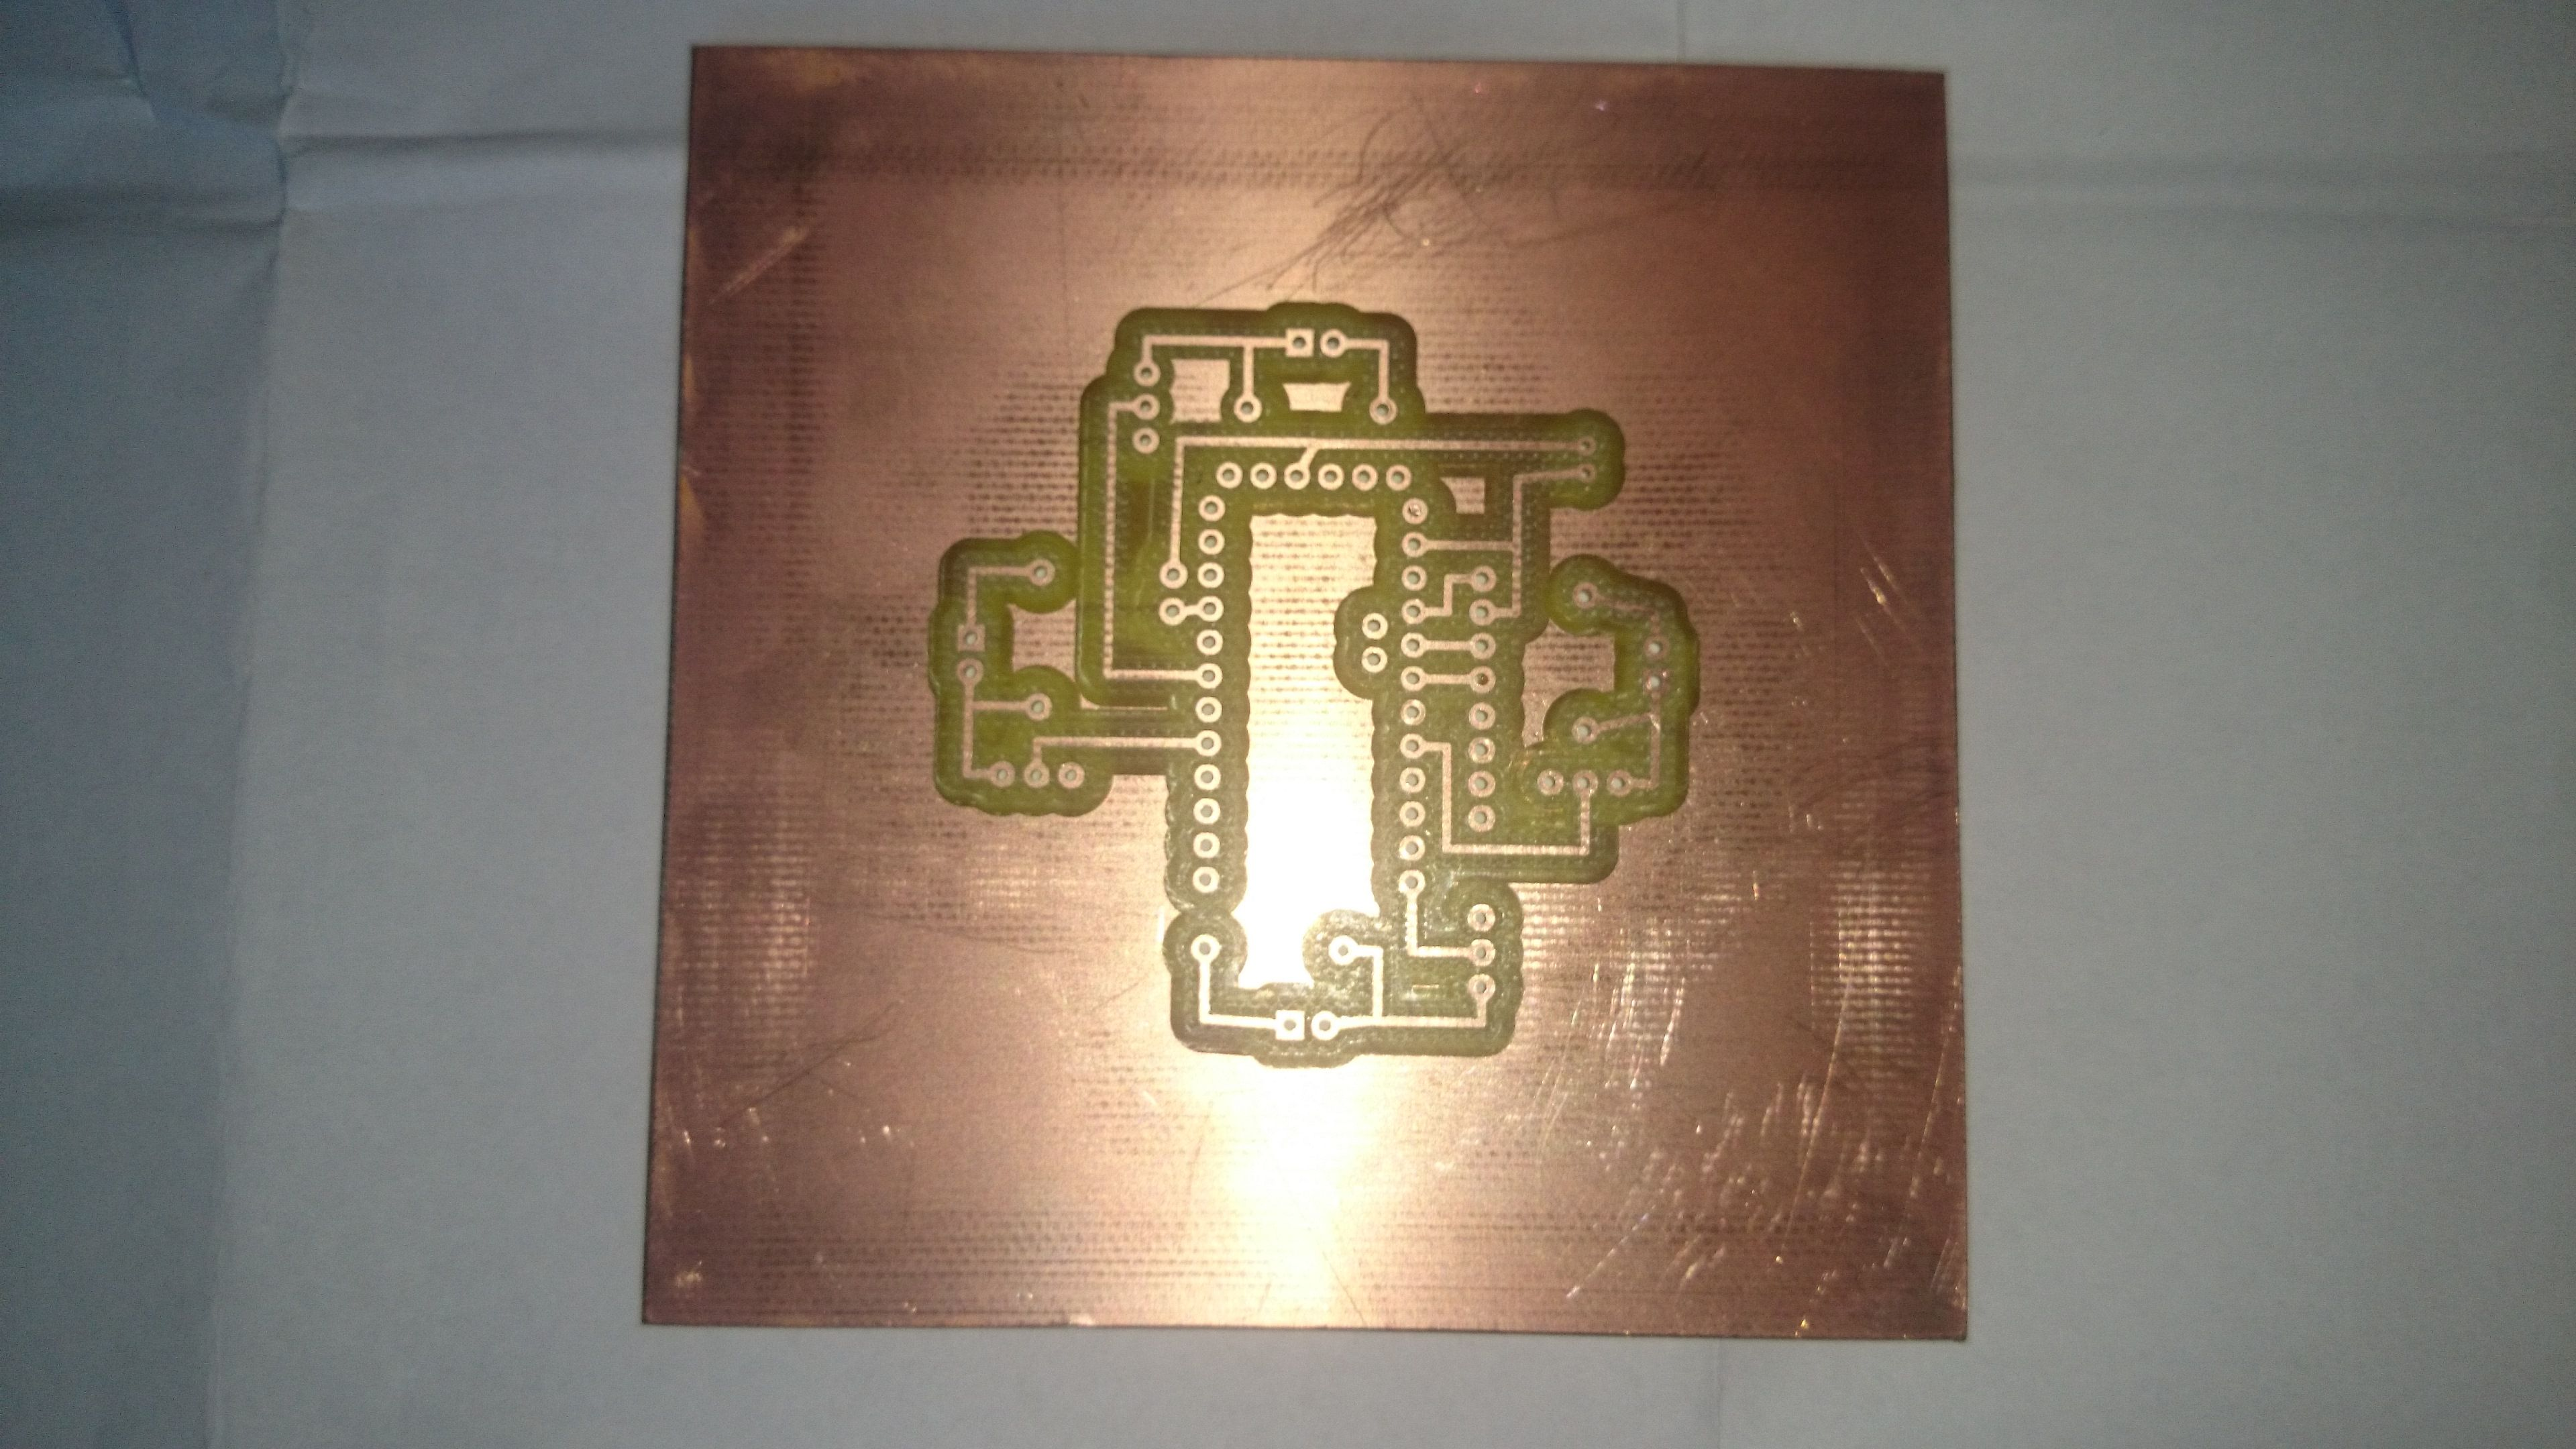
\includegraphics[scale=0.05]{img/carte_avant.jpg}
% 	    \caption{Photo du circuit}
% 	  \end{figure}
	    \begin{figure}
	      \begin{subfigure}{.5\textwidth}
		\centering
		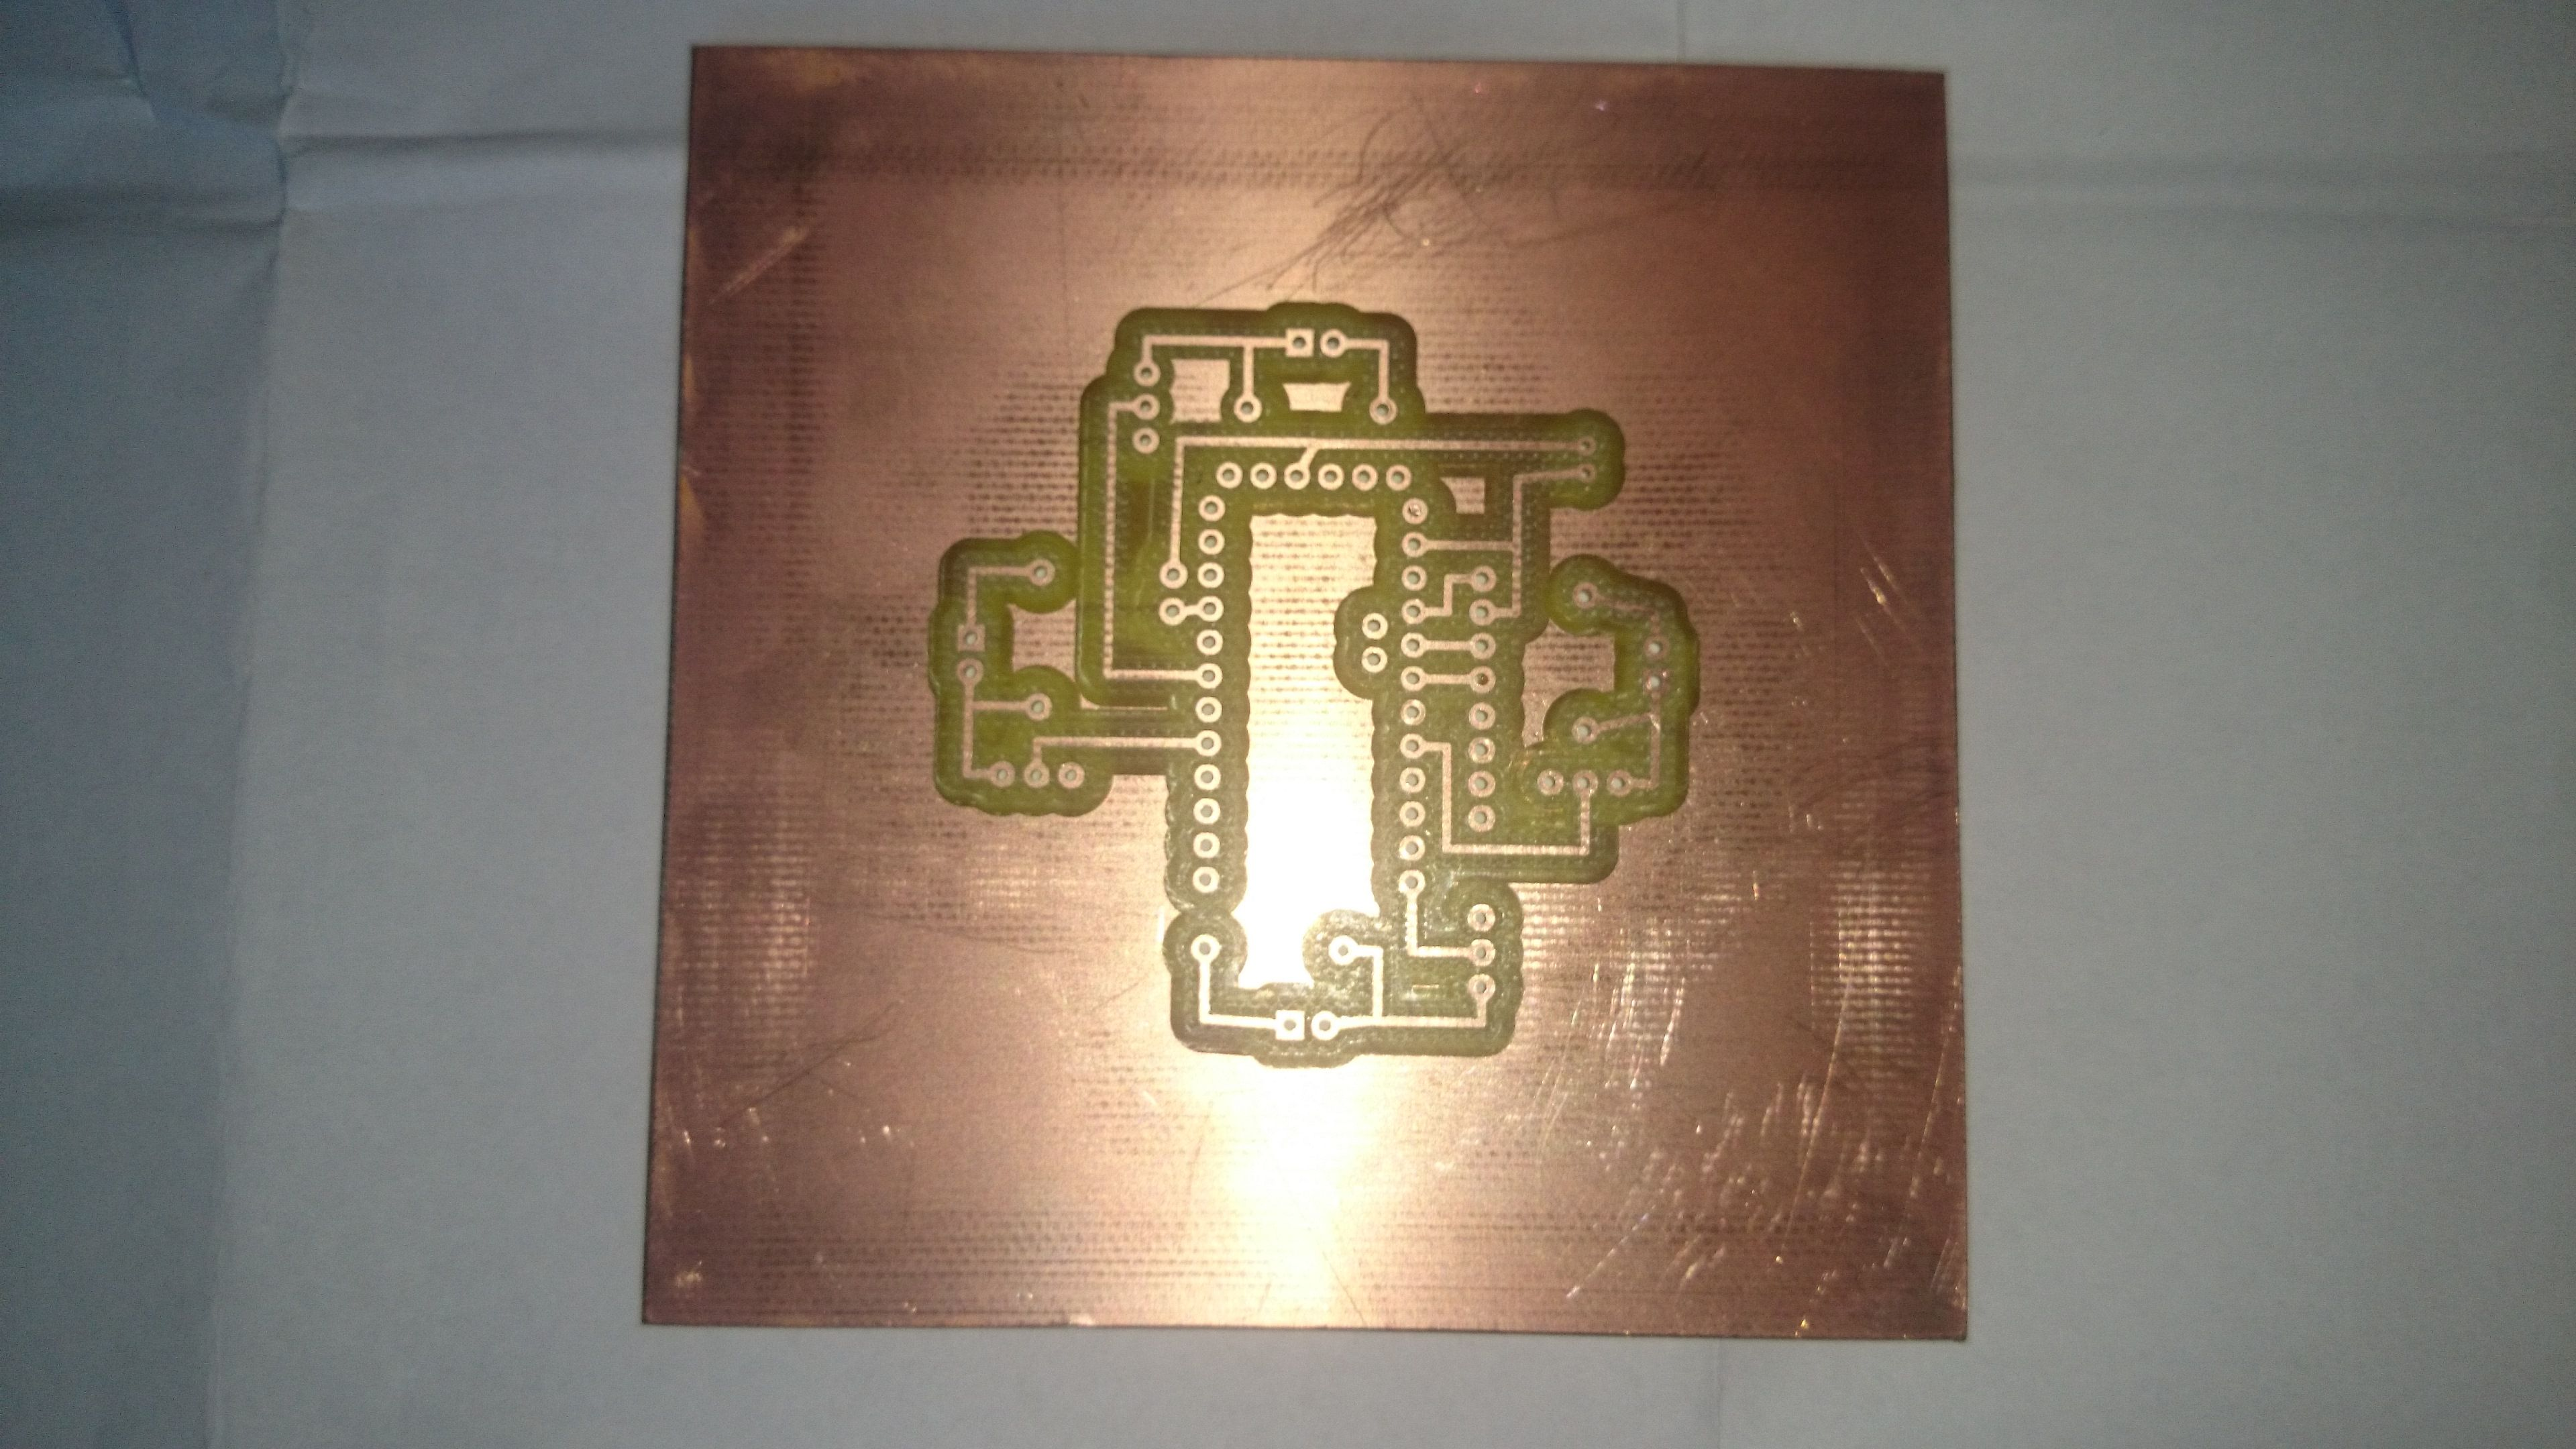
\includegraphics[scale=0.04]{img/carte_avant.jpg}
		\caption{Avant}
		\label{fig:sfig1}
	      \end{subfigure}%
	      \begin{subfigure}{.5\textwidth}
		\centering
		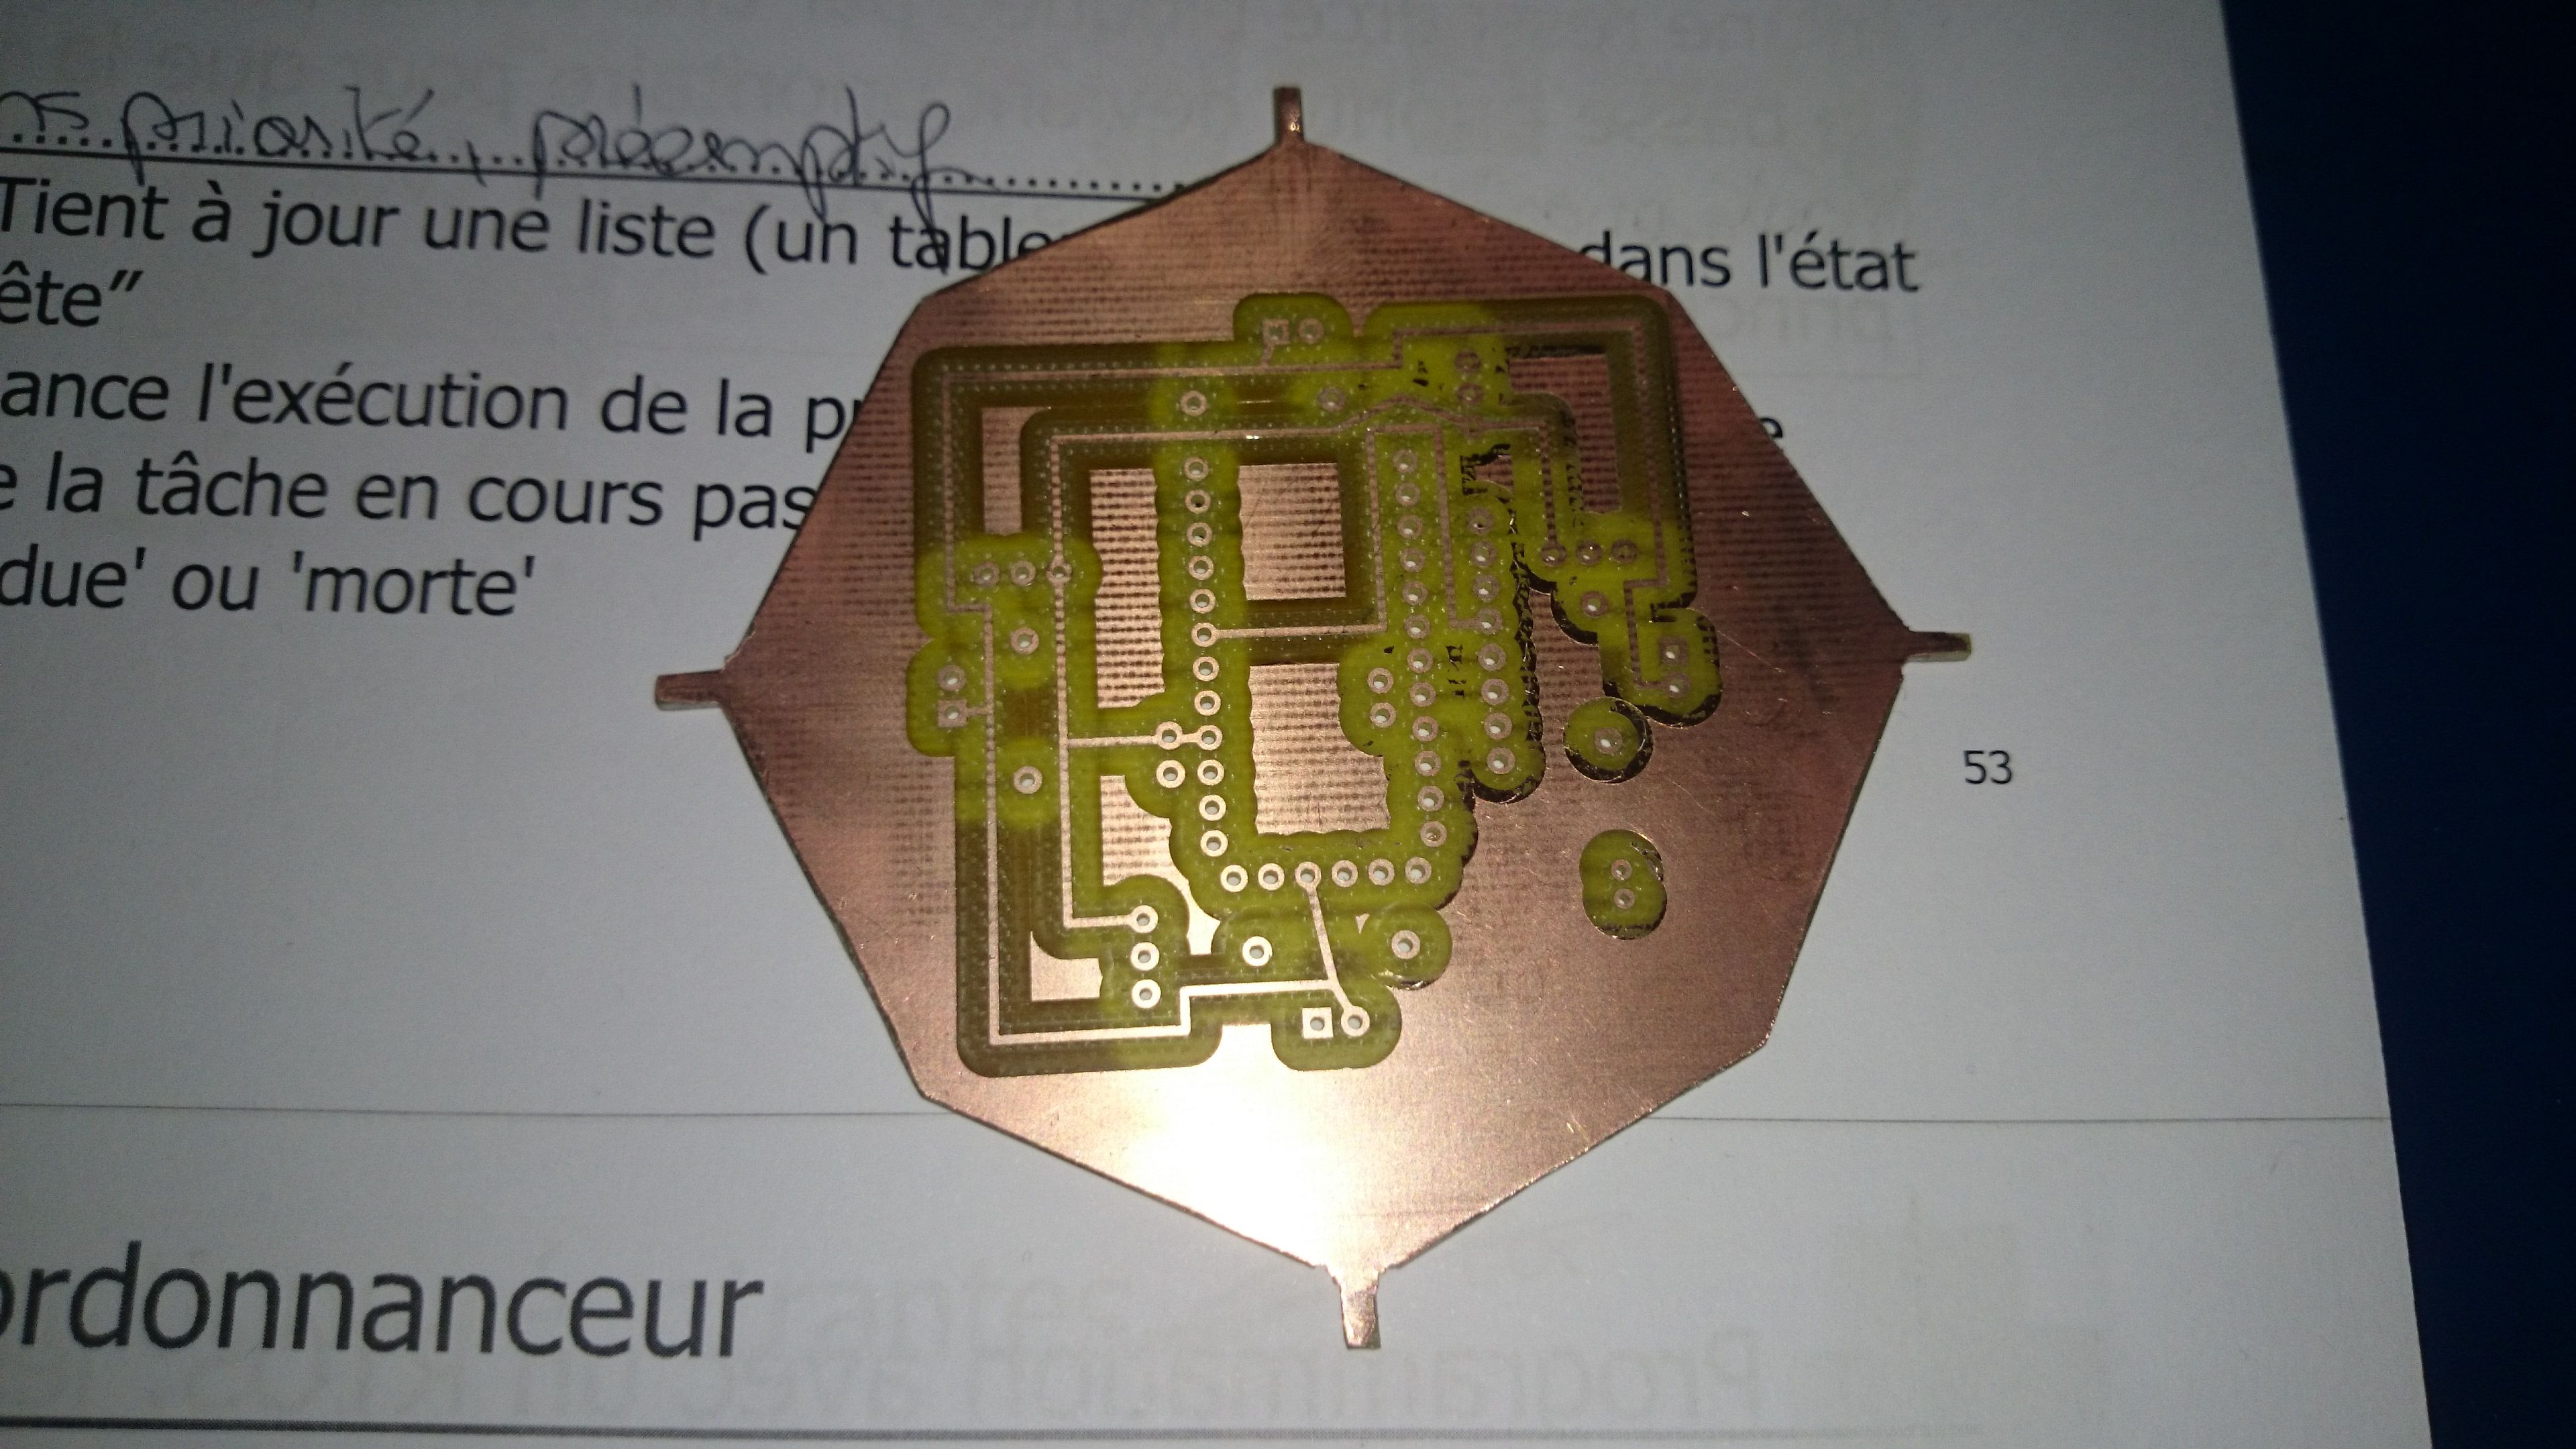
\includegraphics[scale=0.04]{img/carte_apres.jpg}
		\caption{Après}
		\label{fig:sfig2}
	      \end{subfigure}
	      \caption{Circuit avant et après découpage}
	      \label{fig:fig}
	    \end{figure}
	  \end{frame}
	
	\begin{frame}
	  \frametitle{Fixations moteur}
	  
	  \begin{itemize}
	    \item Modèle des pièces disponible sur GitHub
	    \item Demande auprès d'une entreprise, mais pièces trop minutieuses
	    \item Demande auprès de Polytech Instrumentation (filiale de Jeulin) lors de Robafis
	  \end{itemize}
	\end{frame}

	\begin{frame}
	  \frametitle{Fixations moteur}
	
	  \begin{figure}[htbp]
	    \centering
	    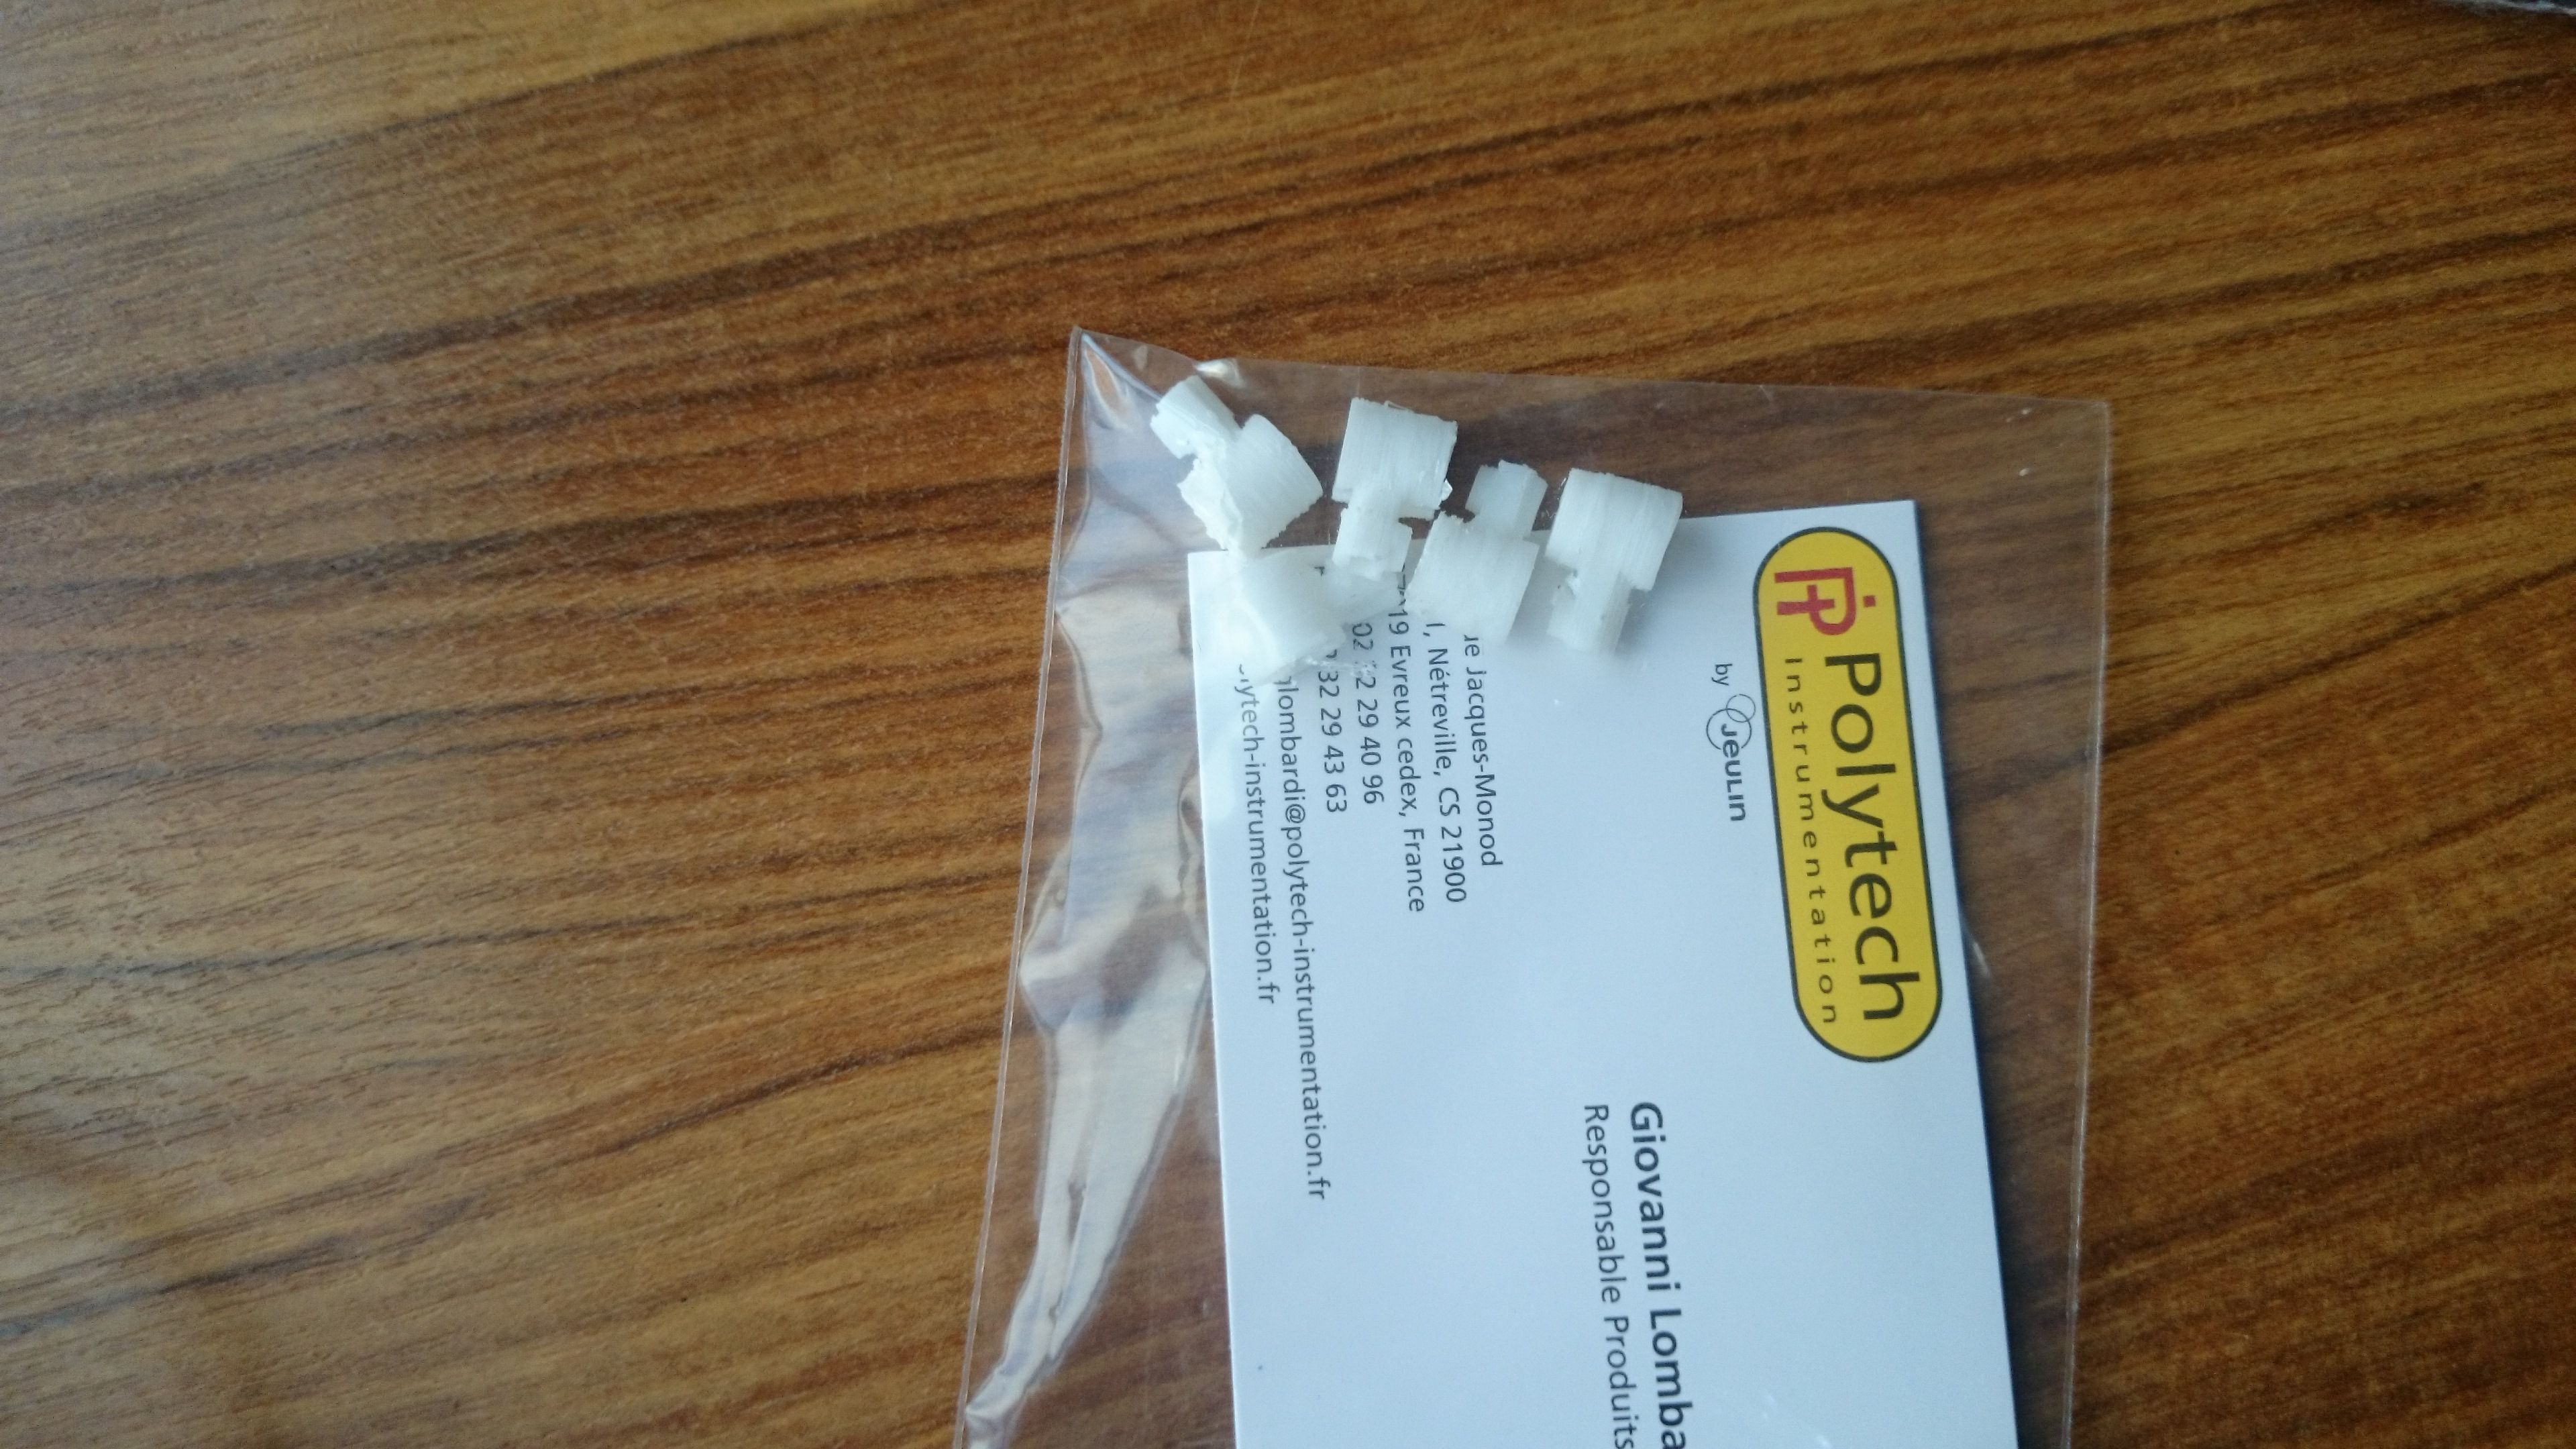
\includegraphics[scale=0.05]{img/fixations.jpg}
	    \caption{Photo des fixations moteur}
	  \end{figure} 
	\end{frame}
      
      \subsection{Résultat final}
	\begin{frame}
	  \frametitle{Après assemblage}
	  
	  \begin{figure}[htbp]
	    \centering
	    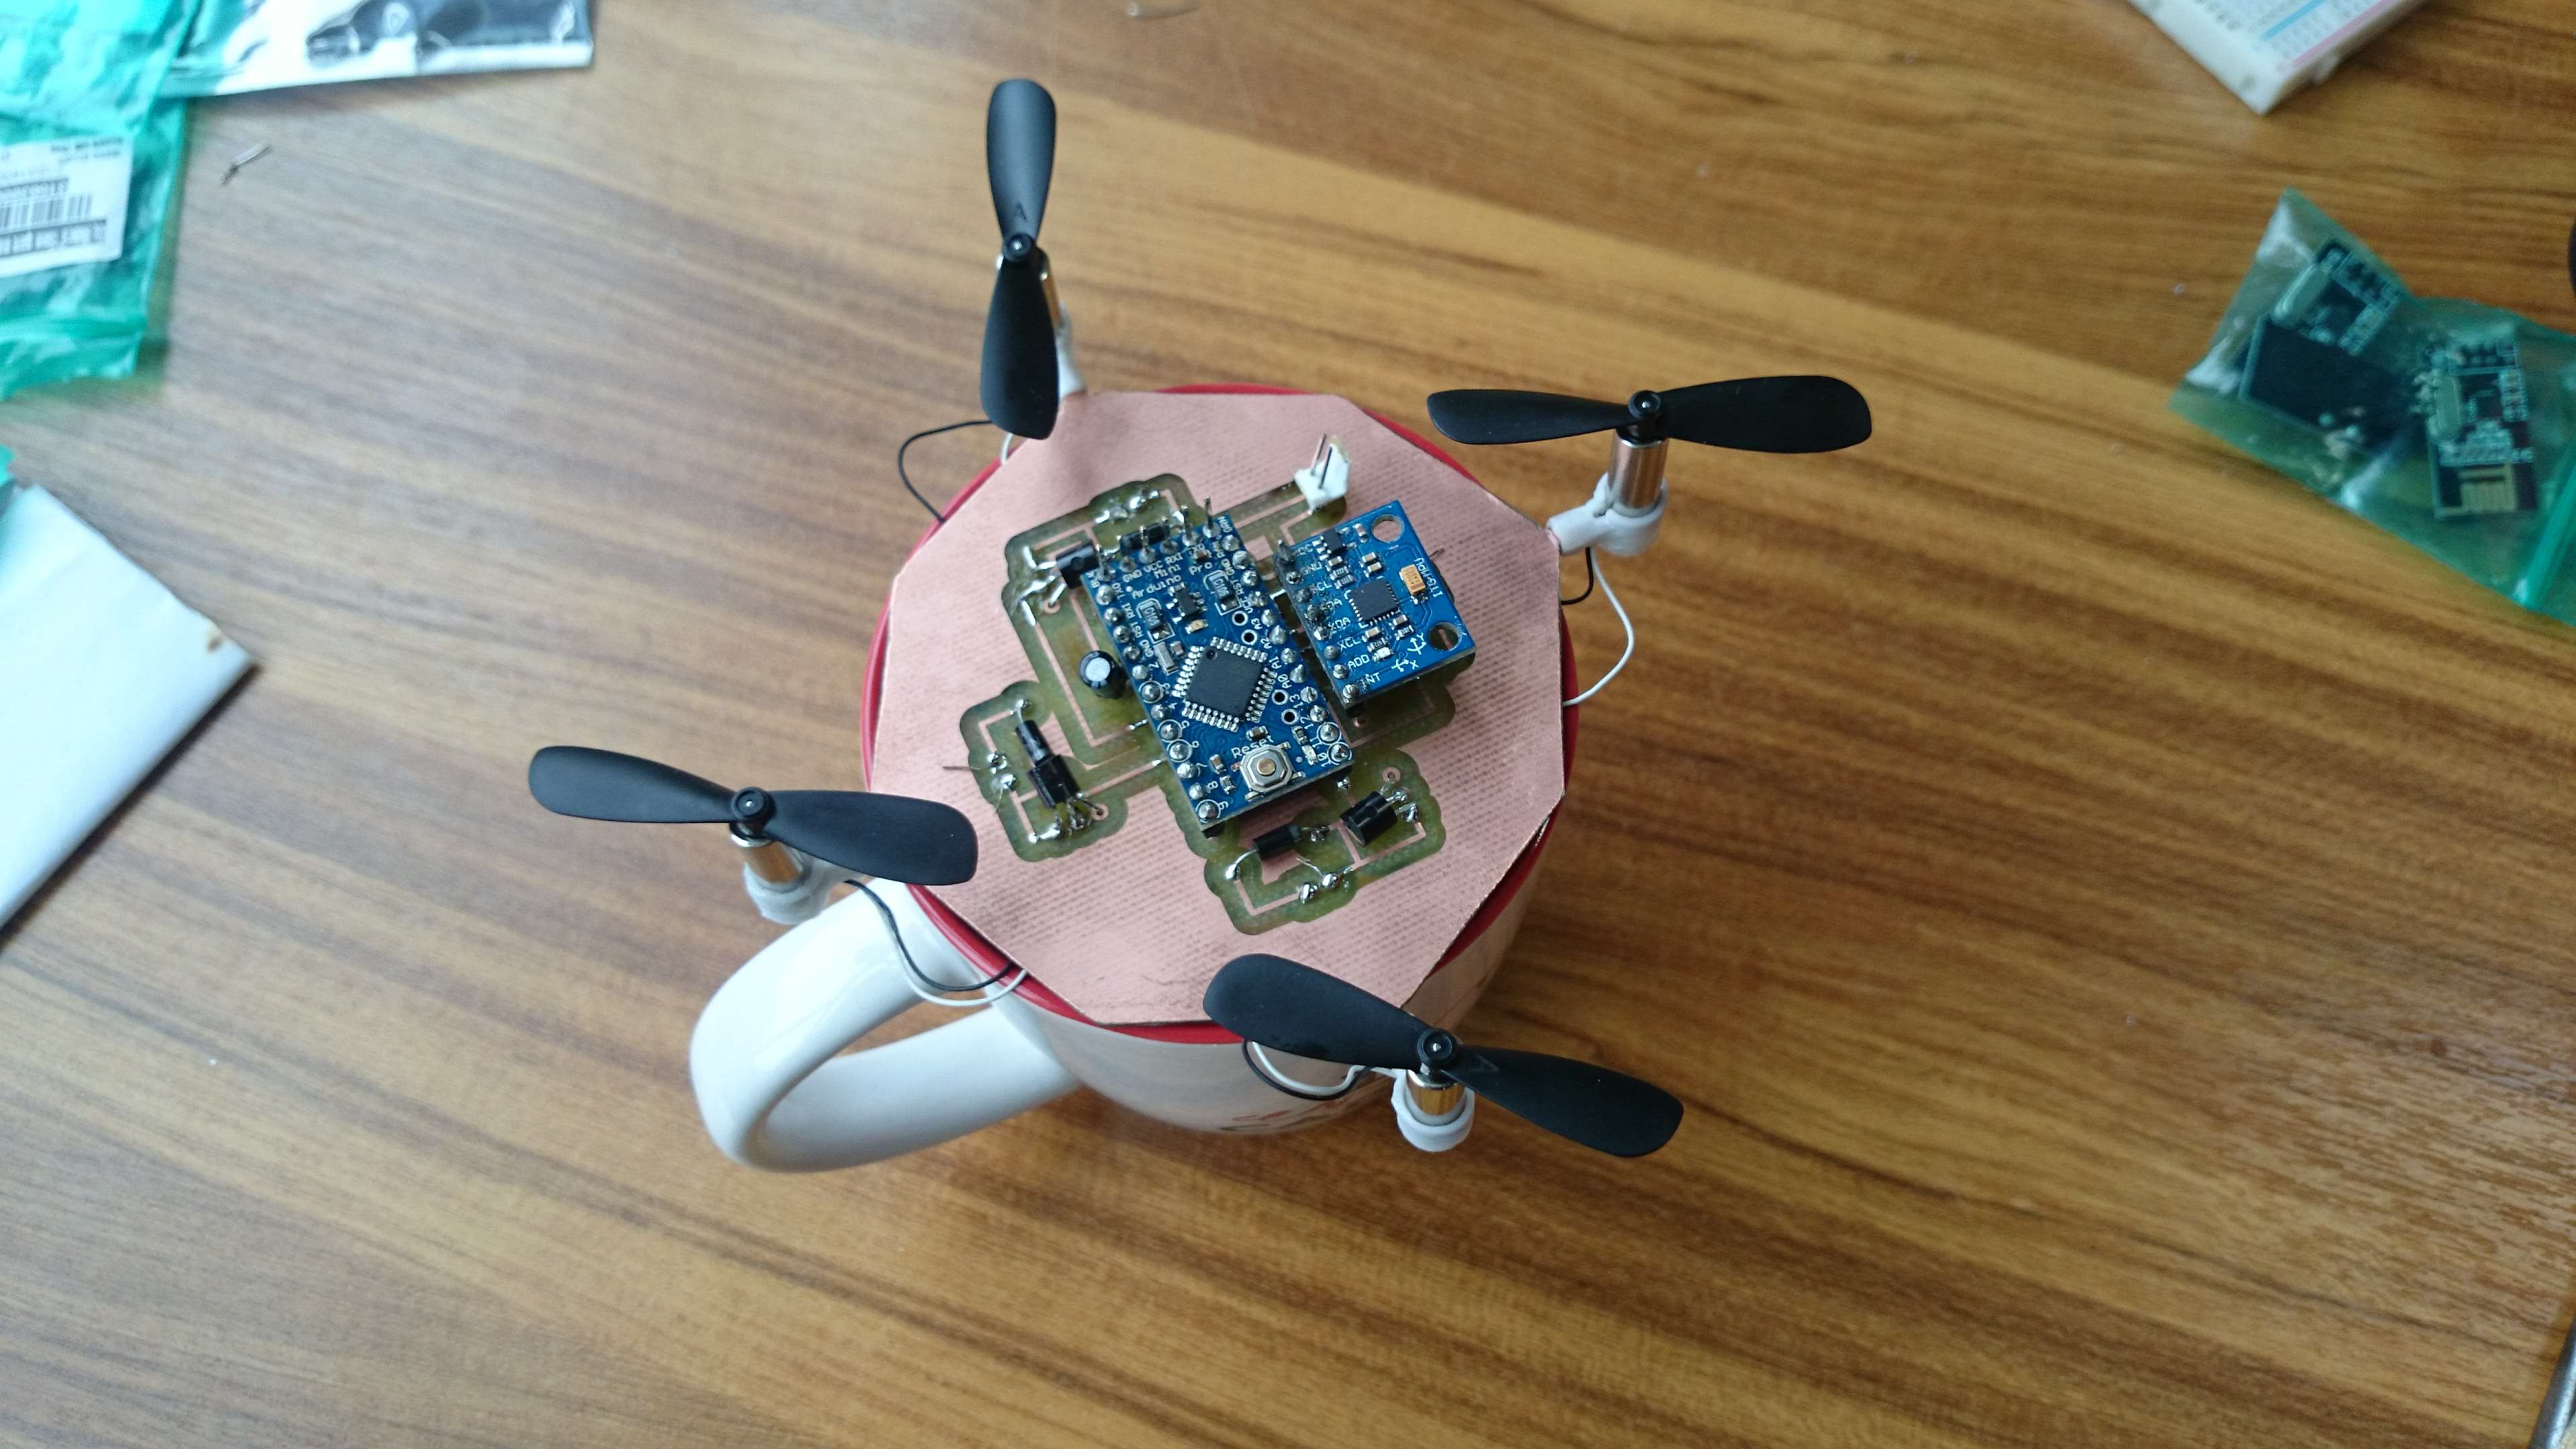
\includegraphics[scale=0.05]{img/drone_photo.jpg}
	    \caption{Photo du drone après assemblage}
	  \end{figure} 
	\end{frame}
	
	\begin{frame} %Test après assemblage
	  \begin{itemize}
	    \item Premier réflexe : Vérifier le décollage
	    \item Plusieurs problèmes
	    \begin{itemize}
	      \item Contrôle moteur depuis l'Arduino : Non suffisant, capacité maximum des moteurs non atteinte
	      \item By-pass de l'Arduino : Peut-être suffisant, un moteur défecteux
	    \end{itemize}
	  \end{itemize}
	\end{frame}
	
	\begin{frame} %Démonstration en direct
	  \makebox[\linewidth]{Démonstration}\par
	\end{frame}
  }
  
  %Section Analyse
  {
    \section{Analyse}
    
      %Re situe le cours de la présentation
      \begin{frame}
	\tableofcontents[hideothersubsections]
      \end{frame}
      
      %Sous-section Conception
      %Aborder les erreurs faites au moment du choix des composants
      \subsection{Conception}
	\begin{frame}
	  \begin{itemize}
	    \item Erreurs dès le devis
	    \item Estimation du poids (approximations et éléments négligés)
	    \item Circuit imprimé élément le plus lourd
	    \item 10\% de la somme totale des composants éléctroniques
	  \end{itemize}
	\end{frame}
	
	\begin{frame}
	  \begin{itemize}
	    \item Choix des moteurs
	    \item Rapides mais couple insuffisant
	    \item Ne peuvent pas supporter le poids du drone
	  \end{itemize}
	\end{frame}
	
	\begin{frame}
	  \begin{itemize}
	    \item Moteurs : alimentés en 3,3V
	    \item Capteurs ultrasons : nécessitent du 5V
	    \item Drone non fonctionnel dès la conception
	  \end{itemize}
	\end{frame}
	
      %Sous-section Contacts extérieurs
      %Parler des différents problèmes engendrés par facteurs qui ne dépendent pas de nous
      \subsection{Contacts extérieurs}
	\begin{frame}
	  \begin{itemize}
	    \item L'EISTI peu adaptée à ce genre de projet
	    \item Besoin de support extérieur (fixations moteur, circuit imprimé, découpe)
	    \item Temps de recherche + création => Délai conséquent
	    \item Premiers essais trop proches de la deadline (fin février)
	    \item Pas le temps de profiter de l'expérience aquise pour une seconde version
	    \item Date de tests idéale : Fin 2014
	  \end{itemize}
	\end{frame}
	
	\begin{frame}
	  \begin{itemize}
	    \item Source d'achat des pièces 
	    \item Coût réduit se ressent sur la qualité (contrefaçon)
	    \item Moteur provenant du même fournisseur, mais puissance différente
	    \item Arduino différente de l'officielle, prise de retard
	  \end{itemize}
	\end{frame}
	
      %Sous-section Montage
      %Aborder les problèmes engendrés par le montage que nous avons fait
      \subsection{Montage}
	\begin{frame}
	  \begin{itemize}
	    \item Faire du circuit, notre châssis
	    \item Deux inconvénients majeurs
	    \begin{itemize}
	      \item Fiabilité de la fixation
	      \item Moteurs non parfaitement verticaux
	    \end{itemize}
	  \end{itemize}
	\end{frame}

      %Sous-section Expérience
      %Parler de notre manque d'expérience pour ce genre de projet
      \subsection{Expérience}
	\begin{frame}
	  \begin{itemize}
	    \item Formation assez généraliste
	    \item Nous ne sommes pas de vrais ingénieurs système
	    \item Projet complexe et nécessite plus de temps (au moins deux ans)
	    \item Contraintes auxquelles nous ne sommes pas habitués (matériel, délai de livraison, système)
	  \end{itemize}
	\end{frame}
  }
  
  %Section Conclusion
  {
    \section{Conclusion}
    
      %Re situe le cours de la présentation
      \begin{frame}
	\tableofcontents[hideothersubsections]
      \end{frame}
    
      \begin{frame}
	\frametitle{Implémentation}
      
	\begin{itemize}
	  \item Création d'une organisation sur GitHub (https://github.com/NjordProject)
	  \item Découpage de l'ensemble du projet en plusieurs sous-répertoires
	  \item Hébergement d'un blog (http://njordproject.github.io/)
	  \begin{itemize}
	    \item français, anglais, japonais
	    \item Suivi du projet
	    \item Ressources pour d'autres projets
	  \end{itemize}
	  \item Utilisation de technologies différentes
	  \begin{itemize}
	    \item Arduino (hardware, software)
	    \item Python (Numpy, MatPlotLib)
	    \item Redis
	  \end{itemize}
	\end{itemize}
      \end{frame}
      
      \begin{frame}
	\frametitle{Serveur}
	
	\begin{itemize}
	  \item Quasiment fonctionnel
	  \item Nécessité d'un drone fonctionnel
	\end{itemize}
      \end{frame}

      \begin{frame}
	\frametitle{Construction d'un drone}
	
	\begin{itemize}
	  \item Challenge énorme
	  \item Connaissances pluridisciplinaires et complexes
	  \item Petites erreurs trop nombreuses
	  \item Manque de temps pour profiter de l'expérience aquise
	\end{itemize}
      \end{frame}
      
      \begin{frame}
	\frametitle{Détermination de la position}
	
	\begin{itemize}
	  \item Grande étendue en extérieur : GPS
	  \item Pièce : Peu de solution
	  \item Problématique au stade de la recherche
	\end{itemize}
      \end{frame}

      \begin{frame}
	\frametitle{Expérience aquise}
	
	\begin{itemize}
	  \item Enrichissant techniquement parlant
	  \item Mais aussi du point de vue relationnel
	  \item Support de la part de contacts extérieurs
	  \begin{itemize}
	   \item Nga Nguyen : Participation de Polytech Instrumentation
	   \item Besma Zeddini : Participation de l'ENSEA
	  \end{itemize}
	  \item Merci !
	\end{itemize}
      \end{frame}
  }
  
  \makeatletter
  \setbeamertemplate{headline}[default]
  \def\beamer@entrycode{\vspace*{-\headheight}}
  \makeatother
  \begin{frame}
    \makebox[\linewidth]{Merci pour votre attention}\par
  \end{frame}

\end{document}
